% vim: set foldmethod=marker:
\documentclass[12pt]{article}
% Packages{{{
\usepackage[margin=1in]{geometry} 
\usepackage{amsmath,amsthm,amssymb}
\usepackage{textcomp}
\usepackage[makeroom]{cancel}
\usepackage{hyperref}
\usepackage{mathtools}
\usepackage{listings}
\usepackage{soul}
\DeclarePairedDelimiter\floor{\lfloor}{\rfloor}
\DeclarePairedDelimiter{\ceil}{\lceil}{\rceil}
\newcommand{\N}{\mathbb{N}}
\newcommand{\Z}{\mathbb{Z}}

%}}}
%Environments{{{ 
\newenvironment{theorem}[2][Theorem]{\begin{trivlist}
\item[\hskip \labelsep {\bfseries #1}\hskip \labelsep {\bfseries #2.}]}{\end{trivlist}}
\newenvironment{lemma}[2][Lemma]{\begin{trivlist}
\item[\hskip \labelsep {\bfseries #1}\hskip \labelsep {\bfseries #2.}]}{\end{trivlist}}
\newenvironment{problem}[2][Problem]{\begin{trivlist}
\item[\hskip \labelsep {\bfseries #1}\hskip \labelsep {\bfseries #2.}]}{\end{trivlist}}
\newenvironment{claim}[2][Claim]{\begin{trivlist}
\item[\hskip \labelsep {\bfseries #1}\hskip \labelsep {\bfseries #2.}]}{\end{trivlist}}%}}}
\begin{document}
\title{EENG 348/CPSC\textsc{338}: Digital Systems}
\author{Kevin Truong \& Rob Brunstad} 
\maketitle
% Introduction {{{
\section{Introduction}
    
    During reading week, students go to Bass Library to concentrate and study
    for their exams. Many students want to study alone and they tend to look
    for one of the individual study rooms as seen in Figure~\ref{room}.
    \begin{figure}[h!]
        \centering
        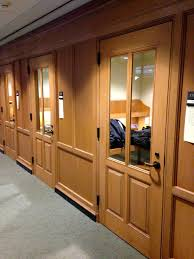
\includegraphics{room.jpg}
        \caption{Individual Study Room in Bass Library}\label{room}
    \end{figure}

    Oftentimes, one has to walk around the whole library to find an empty room.
    This takes around 5 - 10 minutes and sometimes all the rooms are occupied. 
    What if there was an easier and faster way to check if there is a room available
    in Bass?

    The goal of our project is to make an online system which will tell students when a room
    is available and where that room is. We will have LED buttons, as seen in Figure~\ref{button}
    , in each room and whenever a student enters a room, he or she will press the button and 
    the LED will light up and whenever the student leaves the room, he or she will 
    press the button again. The information will be sent to a website which will
    have data about each room and students can easily access the website from there.
    
    \begin{figure}[h!]
        \centering
        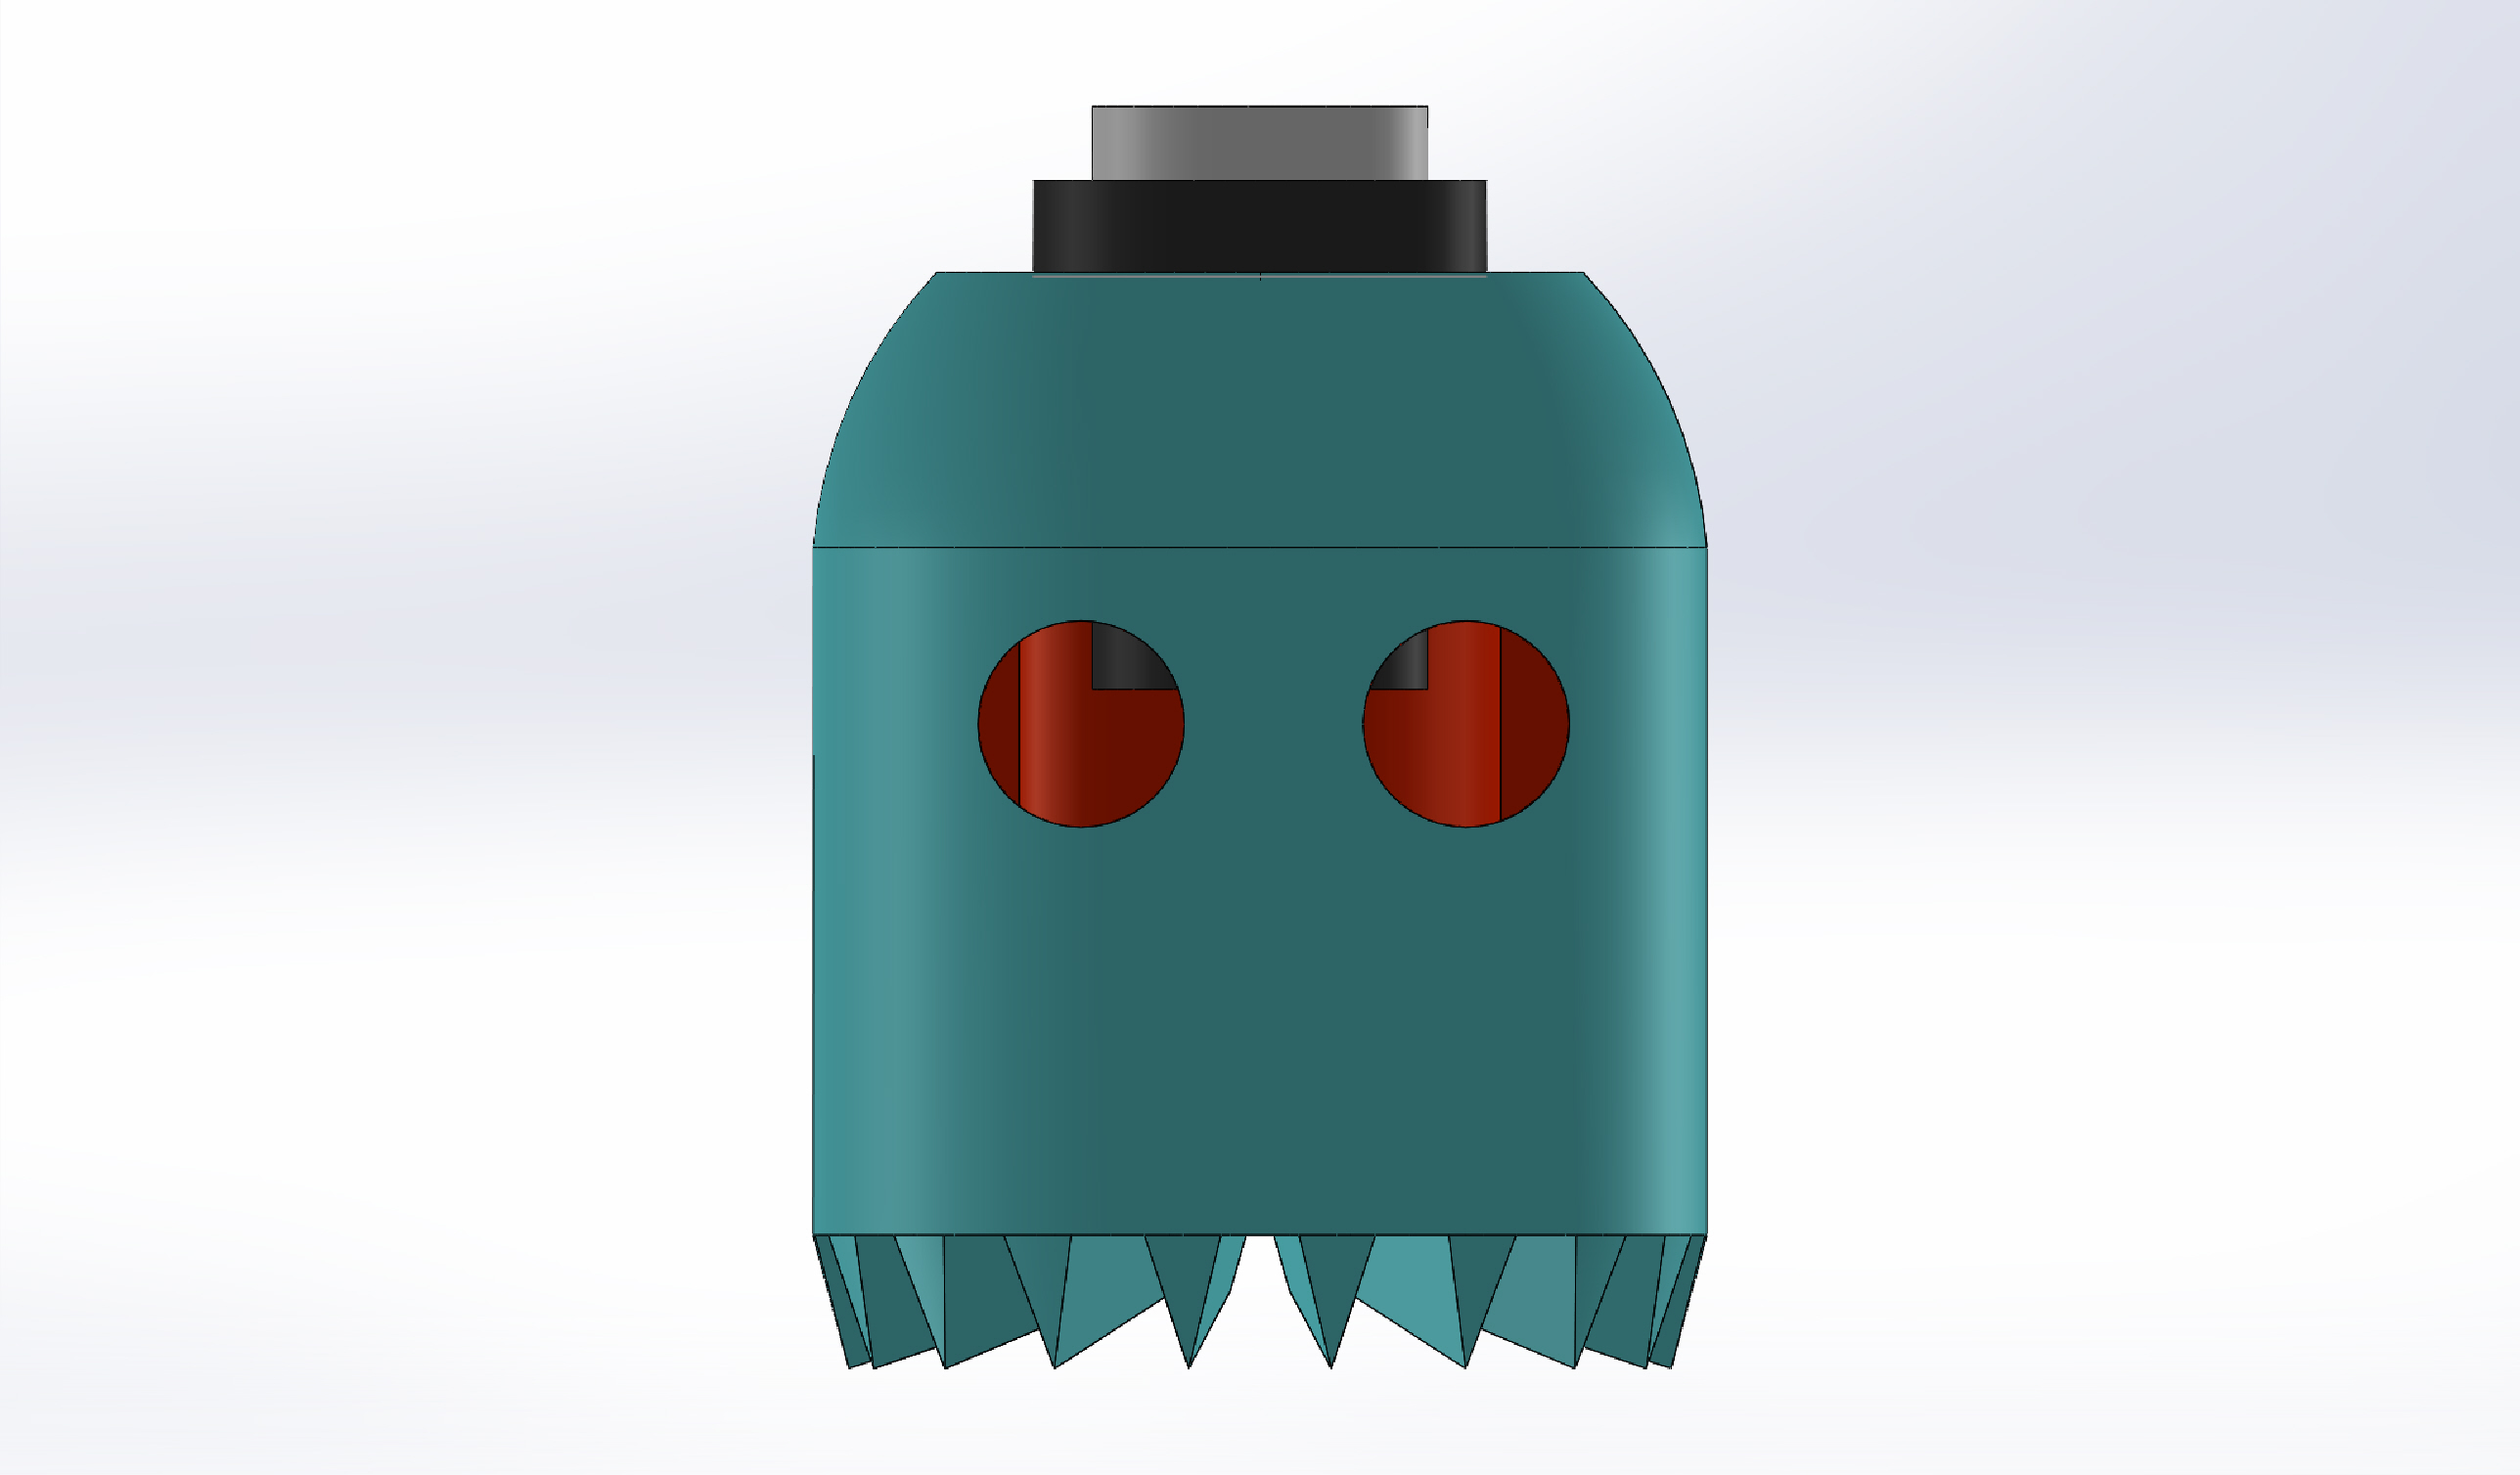
\includegraphics[scale=0.25]{pacman.jpg}
        \caption{3D CAD of LED button with Pacman Design}\label{button}
    \end{figure}

    Each button will be decorated with some sort 3D printed design to incentivize students
    to press the button, similarly to the easy button. We will use the Arduino Nano to send data
    about the button state to the website using the ESP8266 WiFi module. 
% }}}
% Materials {{{
\section{Materials}
\begin{itemize}
    \item \href{https://www.adafruit.com/product/3491}{Arcade Button with LED - 30mm Translucent Clear x 10} 
    \item \href{https://www.sparkfun.com/products/13678}{WiFi Module - ESP8266 x 10}
    \item \href{https://www.amazon.com/Arduino-Elegoo-ATmega328P-without-compatible/dp/B0713XK923}{Arduino Nano x 10}
\end{itemize}
% }}}
% Project Strategy {{{
\section{Project Strategy}
    We plan to 3D print a small container to hold the Arduino Nano and the Wifi module.
    Then we plan to connect the Arduino to a website and get the Arduino 
    to send information about the state of the button to the website. Next we plan
    to make the website as attractive as possible so that students want to use 
    this service since it only benefits them. Finally we hope to deploy these 
    buttons to all of the approximately 50 study rooms in Bass Library.
% }}}
\end{document}
